\chapter{PRE-WTC v0.3}
\setcounter{section}{0}
%%%%%%%%%%%%%%%%%%%%%%%

\textbf{Changelog:}\\
\begin{itemize}
	\item \textit{v0.3} The objective and title again
	\begin{itemize}
		\item \diffdate{2024}{09}{04}{2024}{10}{01}.
		\item Feedback and excellence pieled on, as well as other topics. That it draged on, causes the backlog to swell.
	\end{itemize}
	\item \textit{v0.2} Team Success
	\begin{itemize}
		\item I refocus on the essential element of a rubric, to enabled me to make future decisions. However, to make a decision, it is necessary to have a goal, to evaluated on. Consequently, I am now embarking on this process once more, beginning with the question of what the goal should be.
		\item I got stuck again, and it draged on.
		\item \diffdate{2024}{07}{30}{2024}{09}{01}.
	\end{itemize}
	\item \textit{v0.1} - Responsibilities of Leadership
	\begin{itemize}
		\item In the first cycle 
		 	 \diffdate{2024}{05}{21}{2024}{06}{16}.
		\item There was a side thought: v2 of the concept of an rubric.
		\item In the second cycle 
		 	 \diffdate{2024}{07}{2}{2024}{07}{30}. Mainly in this cycle I was stuck with the collaboration approach. But I was banging my head against the wall. So I rethought it like I did with NFM.
	\end{itemize}
\end{itemize}

\pagebreak

%%%%%%%%%%%%%%




\section{Introduction}

\subsection{Objective}

This topic is written with the goal of outlining the responsibilities, expectations, opportunities, and principles needed to turn a vision into reality with a group of people.

\begin{figure}[H]
	\centering
	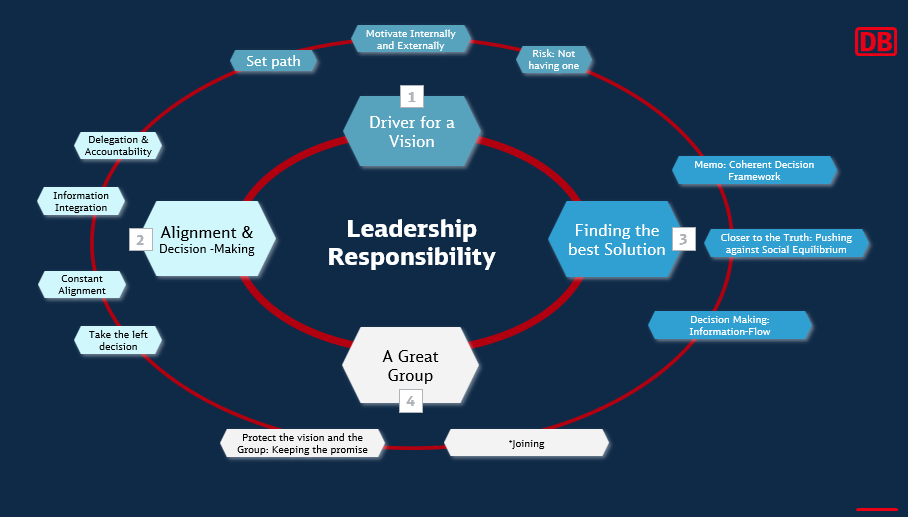
\includegraphics[scale = 0.5]{attachment/chapter_OWN/Rubric_LR_Overview}
	\caption{Key components of the four Responsibility}
\end{figure}

The terms principles and responsibilities will be used interchangeably. As defined in \nameref{Rubic:Prinzip}, these are decision guidelines. Responsibilities can be viewed as predefined tasks, but by linking them with the concept of principles, it becomes clear that these responsibilities also serve a guiding purpose. Additionally, they may help with aligning expectations in the group.

The \gls{p_PRE-WTC} are grouped into four categories, which focus on recognizing and defining responsibilities when pursuing a vision. However, this is not about leadership in the traditional sense, where an organizational unit is managed to ensure the stability of input and output flows. Rather, it is about creating a coherent organizational framework that manages expectations towards others and oneself, allowing individuals to focus on realizing a vision based on their abilities and preferences, by working together as a group.\\

As usual, this is a starting point and does not claim to be definitively correct. However, it should serve as a \gls{p_CDF} when striving to enable a group to consistently provide the best possible solutions and move forward with the vision, and thus requires scrutiny from all sides.

\subsection{Leader and Team, but not really}

All four categories of responsibility are written with a team in mind. However, while approaching the topic, other group dynamics such as alliances, collaborations, and various social dependencies (e.g., expectations, managing the inflow and outflow of members, decision-making responsibilities, etc.) were also considered. The first draft of this rubric (see \ref{sec:Rubric}) failed to establish clear boundaries regarding what constitutes a team and how these principles can be applied across different situations and group structures.

The focus shifted to facilitating a \gls{p_CDF}, thereby increasing the chances of achieving a vision, especially when working with a group of people, independent of if the group is a team or not. However, the general terms are teams and leader, to descript the dynamics and different responsibilities. That states a very simplitice way, of how a group is organised. Hence, the prisms through which the repsonsiblites should be viewed and applied in a given situation requires carfull thoughts.



\section{Four Responsibilities}

\subsection{Driver for a Vision}\label{responsibility__driver}

\paragraph{Set a path: Clear, consistent, constant}

A compelling vision is a prerequisite for \gls{p_PRE-WTC}. This vision aligns with the organization's goals or set's them.\\

This vision serves as a beacon, guiding the team towards a shared future and inspiring them to work together with purpose and enthusiasm.\\

A clear and constant vision helps prioritize efforts and align individual contributions with the broader objectives, both inside and outside the team.\\

It doesn’t need to be explicitly defined in great detail. Explanations can be provided if necessary for decision-making. However, the vision should play a vital role in guiding action and strategy—it’s not a strategy or a plan for achieving it!\footnote{
	In the literature, distinctions are often made between a vision and a mission statement, but the goal here is simplicity: the vision should affect decision-making today and be an integral part of a team or company. For example, a vision can be expressed as a \textit{state} to aspire to, which may typically align with a mission statement, such as \textit{“We are a high-performing digital operation.”} This often indicates a mission rather than a vision. However, in this context, the distinction is irrelevant.
}\\

The responsibility lies in ensuring that this vision is consistently upheld and remains an integral part of the team, influencing decisions and serving as the basis for future projects, strategies, and daily discussions.

\paragraph{Motivate Internally and Externally}
Ensuring social support, capital, and information input for the team to achieve the vision is also part of the leaders responsibility.

\paragraph{Motivate Internally and Externally}
Ensuring social support, resources, and relevant information form outside to help the team achieve the vision is also a key responsibility of leadership.

\paragraph{The Risk: Not having one.}
If the vision is unclear or if the means to achieve it—whether in terms of team capabilities or strategy—are not well thought out, assembling a team becomes risky. The team may fail to move in the intended direction, and the selected skill sets may not be complementary.

If the team achieves great things despite lacking a clear vision, it is likely doing so \textit{despite the leadership}.

\subsection{Alignment and Decision-Making} \label{responsibility__alignment}
This involves turning plans into action, ensuring that the team is aligned and resources are optimally utilized.

\paragraph{Delegation and Accountability}
Delegation is crucial for effective scale.

Based on the required skillset, leaders  the  must delegate (distribute) the responsibilities to right members. This requires knowing the constraint of the group collectivly and an indiviuall level. Also see, who the collectly linking up again

 while holding them accountable forthere outcomes. There are difficulties invole.

and carefully considering constrains. 

As usually this is difficult from the social perspective, because you must work against the desire of group status and harmony.\\

The difference between micromanagement and effective delegation lies in giving team members the autonomy to execute tasks and finding solutions while providing support and oversight as needed, instead of evaluating the solution-finding process, and using once-own way in takeling a given problem. The focus is on evaluating the outcome of once work and how this integrated with other work and the lager vision. 

%TODO: Stop point

Integration and Outcome is key. Both require carful consideration. Thinking about the true desired outcome is

\paragraph{Information Integration} The great team is the best source of information, essesion power and finding the best solutions. In the perfect setting, there individuell work is aligned with the vision. Therefore, they are able to look for alignment problems in the work of there coworkes, that either is in conflict with there owns or with the larger vision. Futhermore, there integrated understanding of the team culture allows them to function as internal feedback-giver.\\

The responsibility lies in using the team to get the best information as possible.

\paragraph{Constantly Align}
Analyzing and gather information about the outcomes of the team is the requirment, to be able to do it
This information should then be used to evaluate progress against the vision or strategy and to constantly communicate what it takes to align actions to achieve it internally and externally. 

\paragraph{Take the left decisions}
$"$Left decision$"$ refers to those crucial choices that no one want or can't make.

That different from "two-door" decisions, meaning they may have a significant impact and are not quickly reversible. If no analytical, logical, or group consensus can be reached for these decisions, leaders must take responsibility and make them. However, the goal is that the group is doing everything, to analysed and make it.


\subsection{Finding the best solutions} \label{responsibility__finding}
This requires nuces for the specific assemble of the team, the field the team is in, and 
% Team Requirement: Deeping on the vison, the field of expertise the team is in.
% Nuces: The assumtion is, that to find the best solution, a lot of comunication, testing, and adapting on new resolts.
% The risk: 
The responsibility, that 
Creating an environment that encourages finding the best solutions is a core leadership responsibility. This involves fostering open communication, promoting collaboration, and encouraging diverse perspectives.

\paragraph{Closer to the Truth: Pushing against Social Equilibrium}
For me, coming closer to the truth is assumtion, what it take for a sucessfull team. There are probably other way to set up culture, and be sucessfull. However, from that are derived responsiblities, that requires, pushing a team and once self out of a social equilibrium, by applieng heuristics, which are design, to foster quick and collective truth finding.   \textit{Note: This equilibrium, must mean, everbody is happy. It means, all action, that a social system took in a given enviroment, are heuristics, which have group cooperation, and group stability as it's funcitional goals. Again: That does not mean, that those heutristic are producing in any enviroment and at any size or time scale a stable group. Further find further explaination, ask the auther.}
\begin{center}
We sacrifice a bit comfort, for a long time success.
\end{center}

\paragraph{Memo: Coherent Decision Framework}
Clear and concise memos ensure everyone is informed and aligned, facilitating better decision-making and coordination.\\

The memo-style presentation of once work is designed, to ensure, to siffout unfinshed thoughts, which a group has to evaluated.
And allow to give persise crital feedback on for e.g. error, different solutions.
This is more work for the autor, but, it should mitegrate the risk of siffing out thoughts, which the autor itself coult done, and using the group abilities, to give target valuable feedback for once work.
As pointed out above, this is not a social heuristic for group stability, just because, this increases the risk for the author to allow a group to find something negativly associated with them. Therefore the responsiblity is, to value the risk, the author took!


\paragraph{Decision Making: Information-Flow}
The goal is not, that all information flows the person leading the group!
The goal is, to have the best decision-making progress, by using each relevant persons inside in improving or finding or stopping a presentated solution TO THE GROUP.\\

Two things are important for this
\begin{itemize}
	\item Arguments should be boucing back to as much as possible of reelvant person. This will required the responsiblity to ensure, people with reservation or general crital options, are encource to speak up, and adressing it as clear as possible.
	\item In reference to \textit{taking the left decisions}. If the leading person estimates, that a decision at the needs to made at the end, then collecting as much as independed information from the group are peramount. For this, the leading person, should talk or make his position clear only at the end. Otherwise, the information flow get's selected beforehand (social eq. heuristic). 
\end{itemize}

This collaborative approach helps surface diverse ideas and fosters innovation.

\subsection{A Great Team} \label{responsibility__great}
The responsiblity lies in that, to find, keep motivated and talented people for the group itself, that they we as a team are most able to fullfill the specifiy vision.

Also the harder responsibility lies in hown the team, that the group itself is protected, by \textit{keep away} pepole are hindering the group in fullfilling the specific vision.

The responsibly lieas, that ties out, that grouopmember goal and aspiration that is aligned with the overall mission. 

\paragraph{To be great, what does it mean?}
In relation to the overall topic of this, it means accomplishing things that are relevant for a great number of people.
Being great in this context does not necessary mean having a great number of skills, which may accomplish something. Nonetheless, having a great skillset may be an indicator of achieving great things in the future.\\

In reference to not having a clear vision and strategy, here lies the risk. People can have a variaty of skills, motivations and potential. Therefore, is paramount, to have a well thought out vision and strategy, to know, what is required to archive it. That's sounds easer then it is. It's very more often then not, clear, what is required.

To that end, the team itself should be guided in finding the best person to fit into the team.

\paragraph{Protect the vision and the Group: Keeping the promise}
% Hone your team
% Focusing attention on the overall goal: Achieving the vision for society and our colleagues themselves.
% If you have to leave, then this should not be a surprise. If the feedback cycle works, then this should be indicated beforehand.

\begin{center}
	If the promise can't or doesn't want to be kept
\end{center}

The promise is that if you join our group, then you are striving to
\begin{itemize}
	\item \textit{align your work to the overall vision},
	\item \textit{towards aligning it to the work of your coworkers},
	\item  and \textit{evaluate your own skills}, to see if they are the right fit right now to serve the team's goals.
\end{itemize}

% If it takes two years to learn specific skills, then you are more than welcome to join again.

If this promise can be kept, then the social harder responsibility\footnote{
	This process is socially hard for the team, the leading person, and the person in question, because
	nobody wants to see somebody suffer, even if it's short-term. Nobody wants to attack a fellow group member, and nobody wants to be excluded. That's what makes it very hard for everybody to go beyond thinking about this topic and actually acting on it.
} is to ensure:
\begin{itemize}
	\item The person in question has to \textbf{leave the team}, or
	\item This person \textbf{must be kept away} from the team, in order to protect the resources and focus, and commitment of the team
\end{itemize}

For evaluation, the team itself should be used for this as well. The responsibility lies in leading the team safely toward this information collection. Safe, because without practice, this is a difficult social area to be in. The upside is that everybody determines and understands what it takes to be part of the team and can reflect on themselves and may counteract before the team has to act.\\

If the leading person sees or deduces from the group behavior that a person can't or won't keep their promise, then this hypothesis should be tested by leading the group to evaluate the situation:
\begin{itemize}
	\item Is a person or are they not keeping their promise in terms of skills, feedback culture, alignment?
	\item Or is this person causing other people to drag with them?
\end{itemize}
If the group clearly states that there is some trade-off or other offset, then either the hypothesis is rejected or the leading person can state to \textit{disagree and commit} with the analysis implication until new information arises.\\

However, if the information collection indicates that the person \textit{should leave} or the team \textit{must be protected}, then the leading responsibility is to make this decision and execute it.





